\documentclass{article}

\usepackage[spanish]{babel}
\usepackage[numbers,sort&compress]{natbib}
\usepackage[T1]{fontenc}
\usepackage[ansinew]{inputenc}
\usepackage{graphicx}
\usepackage{url}

\title{Pr\'actica 2: Aut\'omata Celular}
\author{Anahi Llano}
\begin{document}
\maketitle

\section{Introducci\'{o}n}\label{into}

Se realiza la segunda p\'ractica \cite{elisadyndns} llamada aut\'omata celular
 
\section{Metodolog\'{i}a}\label{met}

Se tomo en cuenta las indicaciones dadas en la p\'{a}gina de la
clase \cite{SatuElisa},realizando ya sea la opcion a)el mayor colapso poblacional o el b)el mayor tiempo continuo de vida en una celda tomando como ejemplo el repositorio modificando el codigo para obtener alguna de las opciones anteriores.

\section{Resultados y discusi\'{o}n}\label{res}

Una vez modificado el codigo y mediante un analisis se pueden observar ambas opciones.
a)para el mayor colapso poblacional, se modifico el codigo de tal manera que nos dijera en cada interaccion cuantos vivios se obtuvieron. \cite{ana} el extracto de datos se puede observar en el archivo "vivosxiteracion" que se encuentra en el repositorio.

\begin{table}
  \caption{Vivos por iteraci\'on}
  \label{t1}
  \begin{center}
    \begin{tabular}{rrr}
      iteracion & \texttt{vivos}
      0 &  93        \\
      1 &  63        \\
      2 &  34       \\
      3 &  26    \\
      4 &  21  \\
      5 &  15 \\
      6 &  12 \\ 
      7 &  8   \\
      8 &  6  \\
      9 &  4  \\
$\vdots$ & $\vdots$ & $\vdots$ \
     50 & 4\\

    \end{tabular}
    \end{center}
  \end{table}
  
En la tabla \cit{t1} se muestra el total de vivos por cada iteracion, se observa que apartir de la iteracion 9 se mantiene estable y son 4 vivos continuos hasta obtener las 50 repeticiones, por lo tanto segun se observa en la tabla \cite{t1} el mayor colapso poblacional fue de 30 celdas que ocurrio al pasar del tiempo 0 al tiempo 1.

Por otra parte para obtener el mayor tiempo de vida igual se realizo una modificacion para mapear las posiciones de los vivos, mandarlos a un text y de ahi una grafica donde se observan en que posiciones se encuentran los que mas se repitieron.

\begin{figure}
  \begin{center}
    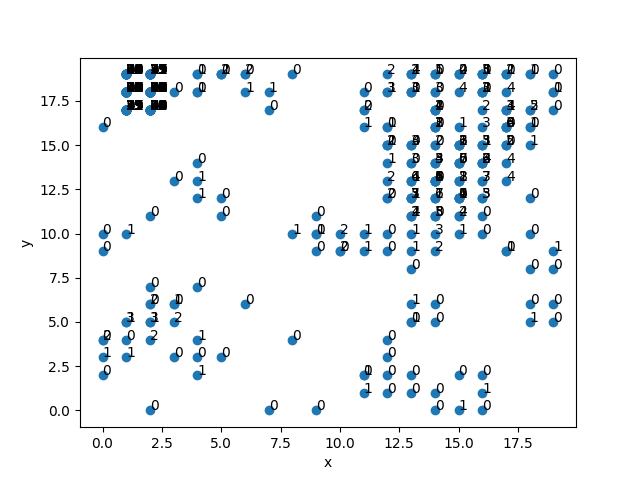
\includegraphics[width=10cm]{posiciones.png}
  \end{center}
  \caption{Mapeo de vivos.}
  \label{f1}
\end{figure}

Mapeando los lugares donde se observa mas negro se muestran las celdas que mas tiempo de vida tuvieron, y para confirmar cuantas itertaciones duraron se observo con busqueda apartir del documento de tex \cite{ana} titulado "mapeovivos" que tambien se encuentra en el repositorio.

\begin{table}
  \caption{Mapeo de vivos.}
  \label{t2}
  \begin{center}
    \begin{tabular}{rrr}
      Fila & \texttt{Columna} & \texttt{Iteraciones que vivio} \\
      2 &  17    & 50     \\
      2  &  18   &  26    \\
      2  &  19    & 25   \\
    \end{tabular}
    \end{center}
  \end{table}
Segun la tabla \cite{t2} que es un extracto de algunos datos que mas se repetian se observa que la celda ubicada en el 2,17 fue la que obtuvo mayor tiempo de vida.
Para observar como se llevaron a cabo las iteraciones se muestra la imagen \cite{ana} "gameover" tambien precente en el repositorio.

\section{Reto#1}\label{ret}

Para el reto 1 se modifico el codigo para simular el crecimiento de grano grueso y obtener la figura en 2D basado en el articulo \ret1 en donde se tomo como inspiracion la ecuacion diferencial para modificar la regla del automata celular. cabe mencionar que en el gif obtenido \cite{ana1} para que se pueda observar una diferencia significativa seria mejor probarlo con un mayor numero de repeticione, por motivos del procesador en la computadora no se pudo correr mas veces.

\section{Reto#2}\label{reto}

para el reto 2 de igual manera se modifico el codigo para obtener una figura en 3D, modificando la regla del automata en este caso no se corrio el codigo ya que seria pesado para la computadora con la cual se trabajo.

  \section{Conclusi\'{o}n}
 Al cambiar la probabilidad inicial de una celda viva conforme al numero de repeticiones, dificilmente puede aumentar el numero de celdas vivas.
El mayor colapso se da en la primera iteracion, y en este caso el mayor tiempo continuo es mas facil observar cuando se cumplen las 50 repeticiones.

  \bibliography{consulta}
  \bibliographystyle{plainnat}
\end{document}